% Legacy predefined pattern coverage from TikZ patterns library.
\usetikzlibrary{patterns}

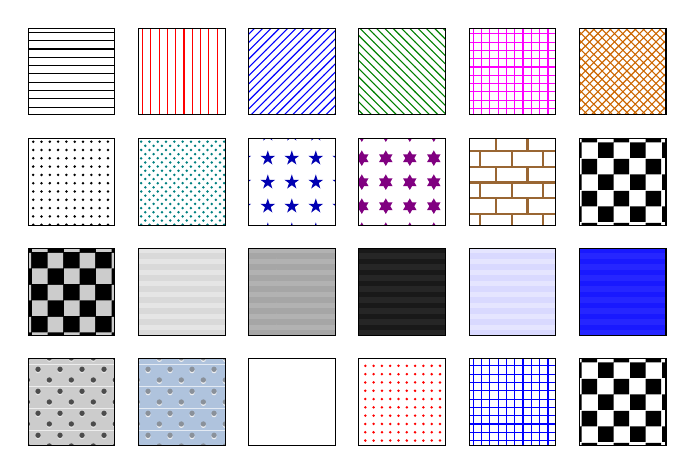
\begin{tikzpicture}[x=1cm,y=1cm,font=\scriptsize]
  % Row 1
  \path[draw,pattern=horizontal lines,pattern color=black] (0,0) rectangle +(1.1,1.1) node[pos=.5] {};
  \path[draw,pattern=vertical lines,pattern color=red] (1.4,0) rectangle +(1.1,1.1) node[pos=.5] {};
  \path[draw,pattern=north east lines,pattern color=blue] (2.8,0) rectangle +(1.1,1.1) node[pos=.5] {};
  \path[draw,pattern=north west lines,pattern color=green!50!black] (4.2,0) rectangle +(1.1,1.1) node[pos=.5] {};
  \path[draw,pattern=grid,pattern color=magenta] (5.6,0) rectangle +(1.1,1.1) node[pos=.5] {};
  \path[draw,pattern=crosshatch,pattern color=orange!80!black] (7.0,0) rectangle +(1.1,1.1) node[pos=.5] {};

  % Row 2
  \path[draw,pattern=dots,pattern color=black] (0,-1.4) rectangle +(1.1,1.1) node[pos=.5] {};
  \path[draw,pattern=crosshatch dots,pattern color=teal] (1.4,-1.4) rectangle +(1.1,1.1) node[pos=.5] {};
  \path[draw,pattern=fivepointed stars,pattern color=blue!70!black] (2.8,-1.4) rectangle +(1.1,1.1) node[pos=.5] {};
  \path[draw,pattern=sixpointed stars,pattern color=violet] (4.2,-1.4) rectangle +(1.1,1.1) node[pos=.5] {};
  \path[draw,pattern=bricks,pattern color=brown!80!black] (5.6,-1.4) rectangle +(1.1,1.1) node[pos=.5] {};
  \path[draw,pattern=checkerboard,pattern color=black] (7.0,-1.4) rectangle +(1.1,1.1) node[pos=.5] {};

  % Row 3 (inherently colored patterns)
  \path[draw,pattern=checkerboard light gray] (0,-2.8) rectangle +(1.1,1.1) node[pos=.5] {};
  \path[draw,pattern=horizontal lines light gray] (1.4,-2.8) rectangle +(1.1,1.1) node[pos=.5] {};
  \path[draw,pattern=horizontal lines gray] (2.8,-2.8) rectangle +(1.1,1.1) node[pos=.5] {};
  \path[draw,pattern=horizontal lines dark gray] (4.2,-2.8) rectangle +(1.1,1.1) node[pos=.5] {};
  \path[draw,pattern=horizontal lines light blue] (5.6,-2.8) rectangle +(1.1,1.1) node[pos=.5] {};
  \path[draw,pattern=horizontal lines dark blue] (7.0,-2.8) rectangle +(1.1,1.1) node[pos=.5] {};

  % Row 4 (remaining inherently colored + pattern=none)
  \path[draw,pattern=crosshatch dots gray] (0,-4.2) rectangle +(1.1,1.1) node[pos=.5] {};
  \path[draw,pattern=crosshatch dots light steel blue] (1.4,-4.2) rectangle +(1.1,1.1) node[pos=.5] {};
  \path[draw,fill=yellow!50,pattern=none] (2.8,-4.2) rectangle +(1.1,1.1) node[pos=.5] {};
  \path[draw,pattern={dots},pattern color=red] (4.2,-4.2) rectangle +(1.1,1.1) node[pos=.5] {};
  \path[draw,pattern={grid},pattern color=blue] (5.6,-4.2) rectangle +(1.1,1.1) node[pos=.5] {};
  \path[draw,pattern={checkerboard},pattern color=black] (7.0,-4.2) rectangle +(1.1,1.1) node[pos=.5] {};
\end{tikzpicture}
